\section{Architektur von Webanwendungen}
Moderne Webanwendungen werden heutzutage überwiegend nach der Client-Server-Architektur aufgebaut. Anders als bei den rein serverbasierten Ansätzen, wird im Client-Server-Ansatz nicht eine komplette Seite im Server generiert und dem Client übermittelt. Stattdessen bekommt der Client initial eine Seite mit wenig Daten, die per asynchrone Aufrufe vom Server geholt werden\cite{Saternos2014}.

Ein Modell dieser Architektur ist die Three-Tier-Architektur, ein dreischichtiges Modell. Hierbei ist die Anwendung in drei logische Schichten unterteilt\cite{Techopedia2017}:
\begin{itemize}
	\item \textit{Tier 1: Präsentationsschicht.} Ist für die Darstellung der Daten und allgemein der Benutzerschnittstelle verantwortlich.
	\item \textit{Tier 2: Anwendungsschicht.} Auch Businesslogik-Schicht genannt, kontrolliert diese Schicht die eigentliche Funktionalität der Anwendung.
	\item \textit{Tier 3: Datenschicht.} Enthält die physische Daten, üblicherweise in einer separaten Datenbank.
\end{itemize}

\autoref{fig:three-tier} veranschaulicht diese Unterteilung der logischen Komponenten im Zusammenhang mit der Trennung von Client und Server.

\begin{figure}[ht!]
	\centering
	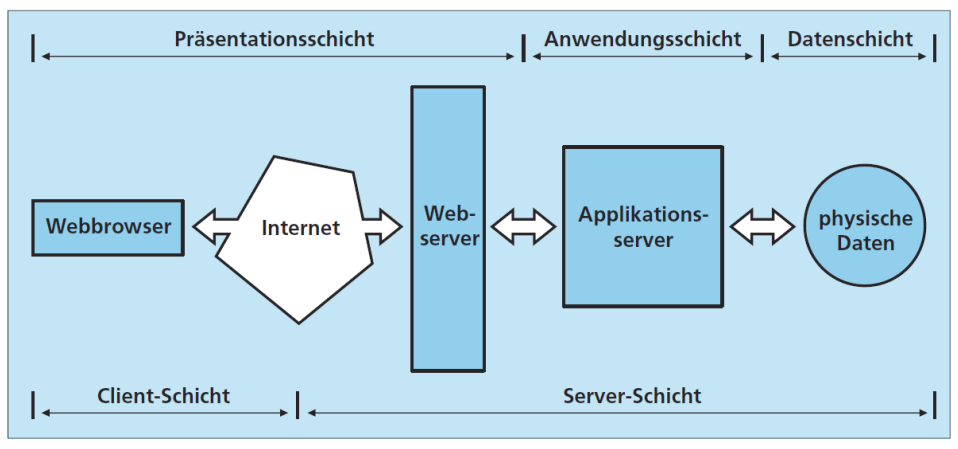
\includegraphics[width=\linewidth]{bilder/kap2/three-tier}
	\caption{Drei-Schichten-Modell der Client-Server-Architektur\cite{Conallen2000}}
	\label{fig:three-tier}
\end{figure}

\subsection{Serverseite}
Sprachen und Technologien

\subsubsection{Webserver}
Was macht ein Webserver? Welche gibt es?

\subsubsection{Applikationsserver}
Was macht ein Applikationsserver? Welche Applikationsserver gibt es?

\subsubsection{Datenbank}
Welche Datenbanken gibt es? Relational, NoSQL + mögliche Produkte
ORM

\subsection{Clientseite}
Sprachen und frameworks

